\documentclass[nochapterpage,bigchapter,linedtoc,longdoc,colorback,accentcolor=tud3b]{tudreport}

\usepackage[stable]{footmisc}
\usepackage[ngerman]{hyperref}

\usepackage{longtable}
\usepackage{multirow}
\usepackage{booktabs}

\hypersetup{%
  pdftitle={Making Matches - Recommending the right personality
  },
  pdfauthor={Paul Schweiger},
  pdfsubject={Personality Recommendation},
  pdfview=FitH,
  pdfstartview=FitV
}

\newlength{\longtablewidth}
\setlength{\longtablewidth}{0.7\linewidth}
\addtolength{\longtablewidth}{-\marginparsep}
\addtolength{\longtablewidth}{-\marginparwidth}

\graphicspath{{g/}}


\title{Making Matches - Recommending the right personality}
\subtitle{Paul Schweiger}

\begin{document}
\maketitle

\chapter{Topic Summary}
As globalization and connectedness advance, online communities grow in importance and the offline world embraces online opportunities. A surplus of possible contacts emerges, making it challenging to have an optimal online experience by engaging with fitting personalities. This interaction between users is a cornerstone of many different activities, such as multiplayer gaming, social networks, crowdsourcing communities or online dating platforms, making matchmaking efforts important to further financial and social goals. Recommender Systems that account for an adequate operationalization of the relevant personality traits can be used to improve said goals all across different domains of usage.\\
The ever-growing market of multiplayer gaming experiences have created online spaces where different personalities are forced to work together. While forming an effective team is the apparent goal of competitive online gaming, for the most part of the community \textit{having fun} is even more important. At the same time, the internet's anonymity makes it a great place for trolls and toxic players, resulting in intra-community problems and a “salty” experience. Not only toxic players, but a combination of different player goals and styles can lead to bad experiences: a single aggressive player in a defensive team will not have the needed support in battle, while players aiming for a story-driven experience won’t be able to cooperate with performance-oriented hardcore gamers.\\
Considering the fact that a large amount of players is available at any given moment, it should be possible to incorporate such preferences in the matchmaking process - which is currently mainly driven by player experience and performance. \\
A recent study by Wang et al. \cite{wang2015thinking} looked at the enjoyment of multiplayer sessions in League of Legends (LoL) based on player personality. They followed a subset of Sternberg's \cite{sternberg1999thinking} problem-solving styles in order to categorize the playstyle of different users. While others tried to gain player personality knowledge by simply asking them \cite{riegelsberger2007personality} or other players \cite{patrick2011system}, Wang et al. automated this process with gameplay statistics. They assigned specific in-game actions to each of their player categories and determined a player's style based on his action profile. Choosing the data used to calculate a "good" experience is highly domain specific and depends on available objective game statistics.\cite{delalleau2012beyond} Match enjoyment for LoL was modeled as a function of game length, with shorter games being less enjoyable due to one team dominating the other.  The results show a clear tendency of specific globally-active and risk-taking players to positively influence the overall game enjoyment. A neural network tasked with predicting match enjoyment achieved better scores when player style data was included, suggesting that this might benefit matchmaking algorithms. However, it is important to note that the used measures are highly subjective to LoL, as interviews with players of both LoL and other games confirm.\\
Most Online Dating Services experience comparable problems: Learning who goes good with one another is a major success criterion for dating applications. Possible matchups need to be built according to their preferences rather based upon global performance. Studies predicting user tastes based on the tastes of similar users, a technique called "Collaborative Filtering", showed better results than global matchmaking. \cite{brozovsky2007recommender}\\
Proper personality-based matchmaking in online environments has a positive influence on overall user satisfaction. Successful Recommender Systems need to incorporate personal and detailed data, rather than just performance measurements. On the other hand the limiting effect of Recommender Systems on content diversity needs to be considered, especially in  this social use case. \cite{nguyen2014exploring}\\

\chapter{Introduction}
The modern world has a plethora of opportunities, topics, people, products, and other things, while people have a limited amount of attention and time to spend. In order to help us guide our attention and resources, basically every digital product tries to recommend meaningful content to users. Recommender Systems play a critical role in modern society and have transcended in many different domains.\\
Online communities grow in importance and the offline world embraces online opportunities. A surplus of possible social contacts emerges, making it challenging to engage with the right person at the right time. QUELLE\\
Interaction between users is a cornerstone of many different activities, such as multiplayer gaming, social networks, crowdsourcing communities or online dating platforms. But besides entertainment, social contacts can also further educational goals.\\
In education research, social and cooperative learning are generally seen as positively affecting learning outcomes. \cite{bossert1982instructional, blumenfeld1996learning} On top of improved cognitive and intellectual performance, successfull group learning efforts can enhance student's skills in other areas, such as the development of social and communication skills and influence the overall satisfaction of students. \cite{zhao2004adding, maxwell2008learning}\\
\textbf{ÜBERGANG IST NICHT SCHÖN. ABSCHNITT KOMPLETT UMSTRUKTURIEREN?}\\
The focal point of technology-enhanced educational research has to improve the individual learning experiences of students by enabling them to engage with richer media or by choosing the right exercises and training sets at the right time, depending on the student's skills, preferences, needs and personality. \cite{drachsler2015panorama, erdt2015evaluating} \textbf{NOCH MEHR HERAUSARBEITEN DASS ES HIER SCHON UM RECOMMENDER SYSTEMS GEHT! GENERELLE RECHERCHEN ZU E LEARNING HABE ICH KAUM!} Furthermore, opportunities for students to receive immediate peer support via online requests have been explored since the earlier days of the internet. \cite{greer1998intelligent} For example, forcing students to discuss their answers to questions in an E-learning environment with their peers led to improvements in both short- and long-term performance. \cite{reidsema2016exploring}\\
The goal of this report is to emphasize how Recommender Systems can be used not to help a single learner to solve problems or improve learning results, but to connect people, to build a community of learners and to enable students to engage in meaningful social learning opportunities. We will take a look at the basics of social recommendations and the importance of reciprocality, will highlight the intricacies of learning group formation and evaluate a recent prototype for reciprocal peer recommendation for learning purposes.\\
Social Recommendation is more complicated, since it needs to account for preferences of more than just a single person. Recommender Systems need account for an adequate operationalization of the relevant personality traits, domain-specific skills and surrounding circumstances.\\
\textit{ALT: This report will discuss possible solutions to improve learning via reciprocal peer recommendation in Learning-Environments. As one of the first (???) and the most recent implementation of such an endeavor, the report will provide a detailed overview of XXXXXXXXX by XXXXXXXX. Important findings leading up towards the work, possible extensions and research in other fields that might prove to be beneficial to this study will be discussed.}\\

\chapter{Related Work: Recommender Systems}
\textbf{SPrachlich scheiße, unübersichtlich, vielleicht nicht nötig?}

\section{User Modeling}
Recommender Systems [RS] are tools that have pervaded our lifes in a lot of different matters. They find use in advertising, e-learning, online-dating, video game matchmaking, social networks, E-commerce, data analysis, and many other topics. The goal of an RS is to emphasize relevant pieces of information in a convoluted stream of data, and to recommend a specific result to a specific user based on his or her history, preferences and situation. \cite{ricci2011introduction}\\
In order to successfully recommend an element, an RS needs to understand its user. The goals, circumstances and domain-specific aspects need to be considered. Thus, RS need to model their users to try and understand what element might be important.\\
Different domains and even different approaches within the same recommendation domain require different user models. For example, multiplayer videogame matchmaking could focus on self-reported preferences \cite{riegelsberger2007personality}, ratings by other players \cite{patrick2011system}, implicit gameplay-derived data \cite{suznjevic2015application, delalleau2012beyond} or a combination of technical and self-reported information. \cite{farnham2009method}\\
A recent study by Wang et al. \cite{wang2015thinking} looked at the enjoyment of multiplayer gaming sessions in League of Legends (LoL) based on player personality. They followed a subset of Sternberg's \cite{sternberg1999thinking} problem-solving styles in order to categorize the playstyle of different users. While others tried to gain player personality knowledge by simply asking them \cite{riegelsberger2007personality} or other players \cite{patrick2011system}, Wang et al. automated this process with gameplay statistics. They assigned specific in-game actions to each of their player categories and determined a player's style based on his action profile. Choosing the data used to calculate a "good" experience is highly domain specific and depends on available objective game statistics.\cite{delalleau2012beyond} Match enjoyment for LoL was modeled as a function of game length, with shorter games being less enjoyable due to one team dominating the other. The results show a clear tendency of specific globally-active and risk-taking players to positively influence the overall game enjoyment. A neural network tasked with predicting match enjoyment achieved better scores when player style data was included, suggesting that this might benefit matchmaking algorithms. However, it is important to note that the used measures are highly subjective to LoL, as interviews with players of both LoL and other games confirm. \textbf{Den Abschnitt hier noch kürzen und geschickt kombinieren mit kleinem Ausblick auf self-reported information. Unten dann bei "besser als self-reported" hier drauf zurück verweisen.}\\
For instance, self-reported information like a user's basic information, preferences or even personality could be considered to improve the user model. \cite{nunes2012personality} This personality data could then be used to find a fitting job for the user \cite{costa1995persons}, or to model a whole group of heterogenous users and to make recommendations based on their shared personality. \cite{recio2009personality}\\
As stated, different approaches fit different problems, although there is naturally some criticism conerning different types of data acquisition. Please reference section \ref{extensions} for a deeper look into this.\\

\section{Social Recommendation}
Since users live in a social world, recommendations can be influenced by social factors or further pervade social spaces. Users might become elements to recommend to others themselves, or connections and networks between users could be used to improve the predicition capabilities of RS.\\
Information about people connected to the current user can be helpful in many different ways. Based on user friendships and shared interests, specific items could that one person liked could be recommended to friends \cite{feng2013recommendation} or just other users with comparable interests to form implicite connections and improve recommendation quality. \cite{hsu2018general} Another approach that was used to enable recommendations with scarce data and mobile computing power was to access a user's contacts and geographic history to find users with matching profiles and more information that can be accessed to improve recommendations. \cite{ramaswamy2009caesar} Or one could use implicite behaviour metrics of many users, like chat engagements on dating platforms, to implicitly derive objective information about a user. \cite{xia2015reciprocal} (This study will be further discussed in section XXX)\\
RS can also be used to recommend social items: other people like in gaming and dating contexts. Research in the educational sector focused on building meaningful professional engagements. A system could, for example, find a supervisor who fits a student's needs in competence, personality and topic expertise. \cite{zhang2016personality} Or one could try to help researchers find meaningful partners on academic conferences based on shared study-interests and personality. \cite{asabere2017improving}\\
\textbf{Passt dieser Abschnitt hier hin?}\\
On a lower level of competency, studying with peers is considered an especially effective way to improve lots of different skills and build knowledge. \cite{maxwell2008learning} When engaging in higher education, many students move to a different town and thus lack a social environment, especially inside their most complicated courses. This makes finding a group a huge initial challenge. Considering the many theories concerning how effective learning groups should be structured (heterogenous with different skill-levels and a minimum joint skill, diverse in terms of gender and ethnicity, ...) \cite{manske2015using, blumenfeld1996learning}, finding an actually helpful group seems to be impossible. This opens another field of study: Peer recommendation in learning. \cite{potts2018reciprocal, olakanmi2017group} [NOCH EINE QUELLE?]\\
Contrary to the aforementioned topics, where often times a specific match for one user had to be found, group learning has to be beneficial for everybody involved. This adds another layer of complexity to this kind of recommendation: Reciprocality.\\
\textbf{Ist die Hälfte hiervon nicht schon Reciprocality?}

\section{Reciprocal Recommendation}
In an extreme case, Recommender Systems will have to recommend users to each other, forming reciprocal recommendations: A user becomes a recommended item and will receive other users as recommendations with the aim to find perfect matches of users who appear in each other's recommendations.\\
TODO: Provide Overview of Reciprocal Recommendation\\
\begin{itemize}
	\item Goal of recirpocal recommendation
	\item different ways to do this: Just a score for other people, or actual reciprocal recommendations, where bothpartners see each other as a recom.
	\item Other fields (Gaming, Dating)
	\item Common methods (Collaborative Filtering)
	\item Common problems encountered when doing this (operationalize personality / relevant aspects, acquire personal information about people, self-reported vs. implicit, ...)
\end{itemize}
Now that the benefits of recommendation in learning, reciprocal peer recommendation and social learning have been established, we can take a look at very recent research combining all of these factors.\\

\chapter{Reciprocal Peer Recommendation for Learning Purposes}
\section{Introduction}
With the goal of providing opportunities for meaningful learning engagements between learners, benefitting mutual success, Potts et al. introduce a novel algorithm and platform for reciprocal peer recommendation in learning environments.\\
The scope of this current study is to demonstrate the capabilities and explore the limitations of such a platform and algorithm on artificial data, before entering it in live conditions. Since the paper was published just recently in March 2018, these further findings are not available yet. However, they are highly interesting: Lots of the theory on peer recommendation in social learning environments needs to undergo detailed testing and research. \textit{Many of the referenced papers are rather theoretical themselves}, or offer insights in different domains and scenarios, making the transfer of knowledge difficult. (BRAUCHE ICH DAFÜR EINE QUELLE? POTTS ET AL SCHREIBEN DAS IN DER EINLEITUNG)\\
This chapter will cover the basics of RiPPLE as a platform and peer recommendation algorithm as well as theoretical findings on artificial data. We will then discuss some shortcomings of the paper at hand, before delving deeper into learnings from other studies and topics that might benefit the overall performance of meaningful peer recommendation.\\

\section{RiPPLE}
RiPPLE ["Recommendation in Personalised Peer Learning Environments"] was designed and developed as a web-based prototype online learning recommendation. RiPPLE is an adaptive, student-facing, open-source platform with the aim to enable students to engage with others in meaningful learning experiences. To enhance the learning experience, RiPPLE functions as a learning platform, helping students to co-create and find meaningful learning-content and to find peers to learn with. This analysis will focus on RiPPLE as a peer recommendation platform.\\
Based on user input, RiPPLE will calculate potential matchups for its users. Depending on the competency derived by a user's performance on learning content, his or her available timeslots and a user's preference on the topics and partner's competency he would like to provide or seek peer support or find a learning partner in, RiPPLE calculates a score for a matchup and will recommend a predefined amount of persons to each user. As RiPPLE currently recommends learning opportunities for the upcoming week, updates to user preferences or competencies are represented once per week.\\
An important aspect of the recommendation algorithm is it's compatibility function, calculating a one-directional score for each combination of potential study partners, u1 and u2. In the first step, the algorithm will check whether a potential matchup is viable following two hard constraints:
\begin{itemize}
	\item a shared timeslot has to be available for both u1 and u2
	\item the topic-specific joint competency must be greater than a prefedined threshold T. According to BLUMENFELD [QUELLE], peer learning sessions will only become effective once the learners can share a minimum understanding of the topic.
\end{itemize}
For every pair of users satisfying these constraints, RiPPLE will calculate the user's respective one-directional scores. These represent how fitting u2 is as a study partner for u1 and vice-versa. (Since the users could have defined different preferences for their competency differences, scores don't need to be symmetric.) The scores take into account how good a matchup will be in terms of overall competency level, and how the other user matches the current users preferences. These calculations will be calculated across all topics relevant for u1 and u2. A visual representation of the resulting score can be seen in figure \ref{f:Seeking}.\\
These two one-directional scores (the score of u2 as a partner for u1 and the score of u1 as a partner of u2,) could now be used to find the the best partner for a specific user. To further recommend a matchup that is beneficial for both u1 and u2, the harmonic mean of both scores is considered as the "reciprocal score" of u1 and u2, a value that is now symmetric. [QUELLE PRABKAHAR 45] The harmonic mean, contrary to the arithmetic mean, pays respect to differences between it's values, making a larger gap between values less desirable. Peer-combinations with approximately similar scores in each direction will receive better final values, pushing matchups that are beneficial to both participants more relevant.\\
\begin{figure}[h]
	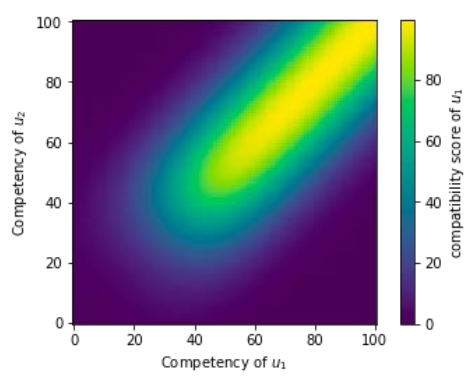
\includegraphics[width=0.5\textwidth]{g/SeekingPartnerCompatibility.PNG}
	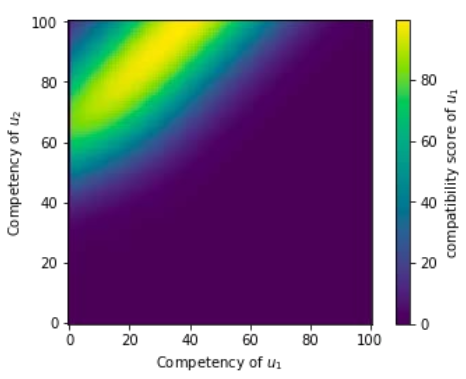
\includegraphics[width=0.5\textwidth]{g/SeekingSupportCompatibility.PNG}
	\caption{The images show the areas of compatibility of a user u2 as a function of u1's competency. Lighter areas mean high compatibility scores in accordance to u1's preferences. On the left u1 is looking for a study partner, leading to the best fit along the u1 = u2 axis. The cutoff beneath a competency of 40 is due to the minimum joint competency threshold T. On the right, we can see u1 looking for peer support, i.e. a person with considerably higher knowledge, here about 60 points higher than u1. Source: \cite{potts2018reciprocal}}
	\label{f:Seeking}
\end{figure}
In the last step, RiPPLE returns a predefined amount of matchups with the best reciprocal values for each user. Although these reciprocal values are now symmetrical, the recommendations don't have to be: While from u1s standpoint the matchup with u2 and an (arbitrary) reciprocal score of 30 could be the very best opportunity, u2 could still have a matchup with u3 and a value of 50.\\
For more information on RiPPLE, the algorithm and further clarification of different variables, please reference \cite{potts2018reciprocal}.\\	
RiPPLE will be evaluated in live conditions in the course of this year. To check whether the implementation could work under real conditions, Potts et al. conducted an evaluation using randomly generated data. This will be discussed in the upcoming section.\\

\section{Evaluation}
In order to test RiPPLE's applicability for actual use, Potts et al. designed an experimental setup in which RiPPLE would try to propose recommendations for randomly generated test data. Specific quality measures were designed to assess different fields in which RiPPLE would have to show its capabilities. With satisfying results, RiPPLE would be able to be used under live conditionsin the course of 2018.\\
\\
To conduct the experimental evaluation, random data had to be generated; diverse enough to highlight edge cases but within reasonable bounds. For a set of 1000 users, 10 learning topics and 10 possible timeslots, each user received a random distribution of relevant values. Topic-specific competencies were expressed as a value from 0 to 100 derived from a truncated normal distribution around a random mean with fixed variance. Each user received competencies for every topic. These were then sorted from low to high, and a random number of these topics were chosen to be part of the user's request. The highest competencies of every user were classified as "providing support" roles, the lowest as "seeking support" and the median topic received a "co-study" role. In absence of empirical data, competency difference preferences were modeled as a fixed value per chosen role, as opposed to a explicitly stated preference for each user. Every "user" was made available during random timeslots.\\
\\
To fully satisfy as a tool to recommend students to one another, Ripple must be able to form meaningful and successful matches for as many users as possible in reasonable time. On the other hand, minor drawbacks in the defined metrics were considered to be tolerable due to the experimental and randomly generated data and some further adjustments that could be made to compensate bad values.\\
As Evaluation Metrics for their experimental evaluation Potts et al. decided on four values that can further be used as general Quality Measures for reciprocal recommendation algorithms:\\

\subsection{Scalability} With increasing enrollment numbers in higher education, RiPPLE will have to be suitable for large sets of learners. High runtime and costs for evaluating datasets with reasonable amounts of students means slower responses and a worse user experience. An optimal solution could provide immediate recommendations to any user, at any moment.\\
As can be seen in figure \ref{f:scalability}, the runtime of the algorithm increased in a quadratic fashion, as U, the total amount of users, increased: \(O(n^2)\). The number of recommendations per user, however, does not significantly impact the runtime. (Although the paper states that it \textit{did} in fact affect runtime, looking at the plotted data suggests that this might be a formatting error.)\\
Currently, RiPPLE calculates recommendations at the end of each week for the upcoming week, making the algorithm's runtime rather unimportant. However, further improvements are planned.\\
In a 1000 user experiment, RiPPLE was able to provide recommendations for a single user in 0.045 seconds - which is a pretty good time.\\
\begin{figure}[p]
	\centering
	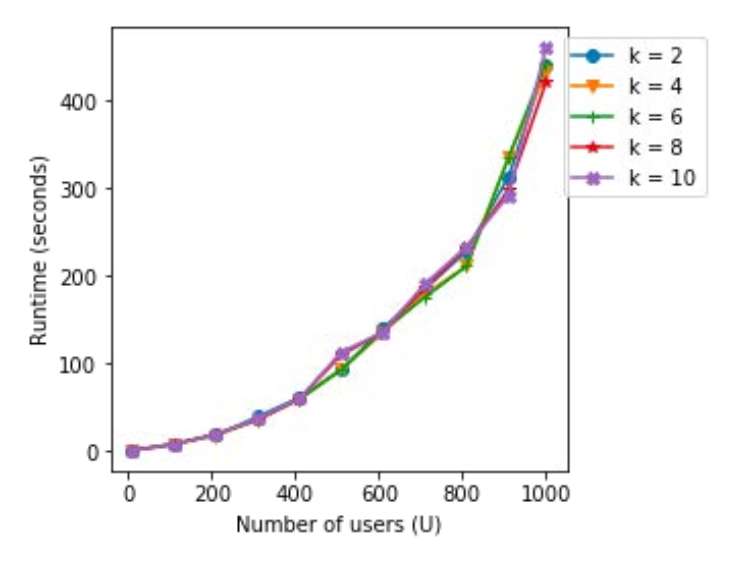
\includegraphics[width=0.5\textwidth]{g/Runtime.PNG}
	\caption{Scalability: The algorithm's runtime depending on the number of users \(U\) and the amount of recommendations per user \(k\). Note how k has almost no influence on the runtime, while it grows exponentially with increasing U. Source: \cite{potts2018reciprocal}}
	\label{f:scalability}
\end{figure}


\subsection{Reciprocality} The best possible recommendations are reciprocal: Users contacting a recommended user would also appear on this user's list of potential study partners. Reciprocality was tested for both, the baseline non-reciprocal and the joint reciprocal average scores. Whenever a user appears in the recommendations of a user on their own recommendation list that was built according to the respective score, the recommendation was considered to be reciprocal.\\
The precision for every user given the used score is calculated by dividing his reciprocal recommendations through \(k\), the total amount of recommendations that user received. The system's total precision is defined as the average precision across all users.\\ 
QUELLE\\
In all tested cases shown in figure \ref{f:reciprocality}, the reciprocal score had a higher precision than the baseline score. This is not surprising, since using the harmonic mean of both one-directional scores chooses reciprocal scores with medium values compared to non-reciprocal scores with a single high value. [REFERENZ AUF ERKLÄRUNGSABSCHNITT] Increasing \(k\) also increases the precision, since more recommendations per user lead to a higher chance of reciprocal recommendations. On the other hand, increasing \(U\) with a fixed \(k\) reduces reciprocal precision, since there are more possible users to recommend.\\
\begin{figure}[p]
	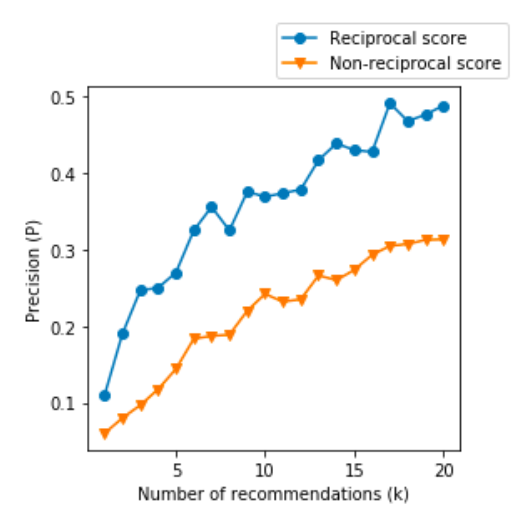
\includegraphics[width=0.5\textwidth]{g/PrecisionByK.PNG}
	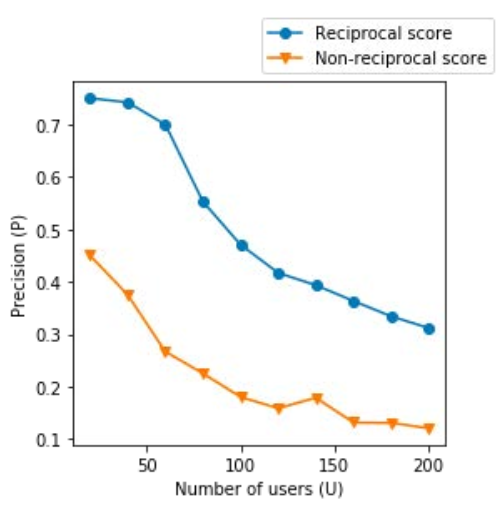
\includegraphics[width=0.5\textwidth]{g/PrecisionByU.PNG}
	\caption{Reciprocality: The precision (= the fraction of reciprocal recommendations out of the total recommendations averaged over all users) of the baseline non-reciprocal recommendations (orange) vs. of the reciprocal, averaged scores. Note how the reciprocal scores are always better. Source: \cite{potts2018reciprocal}}
	\label{f:reciprocality}
\end{figure}

\subsection{Coverage} Recommending potential learning partners to one another should be made for as many users as possible, not abandoning anyone. As such, coverage is a very important metric to consider. Since (almost) every user will receive recommendations, most users will be covered in one way or another. (The exception to this are users with completely incompatible timeslots, role preferences (i.e. being the only person looking for an equally skilled study partner) or users who can't meet the minimum competency when coupled with their available potential partners.) A good fit can only be ensured when the same user is recommended to others, ideally forming a reciprocal recommendation, which is represented in another quality measure. Coverage however is defined as the percentage of users that appear in other's recommendations at least once.\\
For a low amount of users and lots of recommendations per user, coverage is close to 0.9, meaning most users are recommended to others. As U increases or k decreases, the coverage sinks. However, more than 40\% of users appear in other's recommendations under all tested circumstances. Reference figure \ref{f:coverage} for a graphical overview.\\

\begin{figure}[p]
	\includegraphics[width=0.5\textwidth]{g/CoverageUk.PNG}
	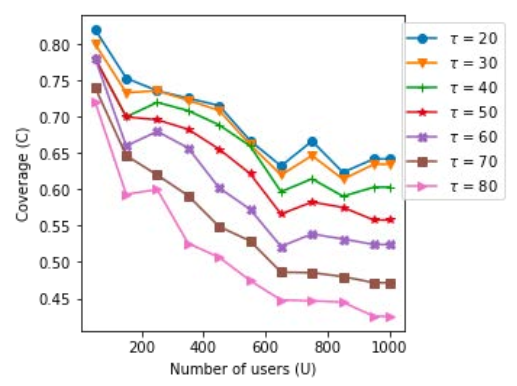
\includegraphics[width=0.5\textwidth]{g/CoverageUT.PNG}
	\caption{Coverage: The percentage of users who appear in other's recommendations. With more users, coverage sinks (likelihood of hard to match users increases). Increasing received recommendations or lowering the minimum joint competency of matches increases coverage. Mind the y-axis cutoff. Source: \cite{potts2018reciprocal}}
	\label{f:coverage}
\end{figure}

\subsection{Quality} The quality of a recommendation is not only based on its fit, but also on how good the resulting team could perform. According to BLUMENFELD QUELLE, learners should meet a minimum competency level in order to be an effective group, as specified by the employed minimum matchup threshold T and leniency factor alpha. [IST ES GUT DIE HIER ZU ERWÄHNEN? HÄNGT DAVON AB WIE ICH DIE BILDER EINBINDE] Quality is thus defined as the user's average joint competencies across their matched topics. The goal is to generate matches, that are as capable as possible in their respective fields of study.\\
Referencing figure \ref{f:quality}, it is apparent that the total amount of users does not affect the quality of matches. The minimum threshold for joint competency of a matchup however leads to a better quality. Comparing this finding to \ref{f:coverage} however, suggests that higher quality comes at the cost of less coverage. Especially when considering the slight improvements in quality score for larger increments in T.\\
\begin{figure}[p]
	\centering
	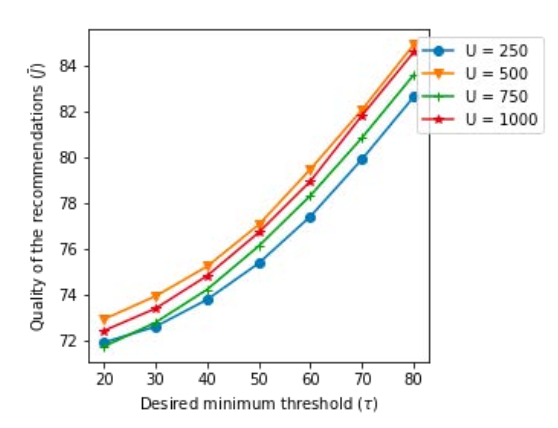
\includegraphics[width=0.5\textwidth]{g/QualityByU.PNG}
	\caption{Quality: The quality of matchups over different values for U and T. Note how changing U won't affect matchup quality. Choosing a higher minimum joint competency threshold T for successful matchups increases overall quality. Note the different scaling of the axes, overemphasizing the quality increases. Source: \cite{potts2018reciprocal}}
	\label{f:quality}
\end{figure}

\section{Discussion} \label{sec:disc}
"Reciprocal peer recommendation for Learning Purposes" and the implemented platform RiPPLE present an approach to build a scalable, interactive and user-facing, multi-purposes learning platform to enhance learning both in on- and offline circumstances. RiPPLE's flexiblity in some threshold values allows the tool to be customised to address some of the shortcomings of peer recommender systems identified by OLAKANMI AND VASSILEVA QUELLE. While the experimental results look promising, further research on actual data has to be conducted, which is planned over the course of the year.\\
Recap of their discussion\\
The experimental evaluation of the platform's performance using artificial data sheds light on variable relationships, potential initial values for scientifically sparse concepts and the interplay of lots of factors. While the values reported from evaluation with artificial data present good metrics to measure the algorithm's performance and suitability for live data, they don't actually evaluate the algorithm, since no targets have been set. Although the data is quantifiable, these findings should not be mistaken as quantitative results: instead of comparing the data to theory-driven goals and evaluating them for actual use, they are more or less providing an overview of how the algorithm works. In fact, there is currently no way to know of these results are "good". \textit{Many of the used measurements lack consistent data and research, and are not theoretically funded.} The question whether a coverage of little above 0.4 will be enough in practice, remains unanswered. Actual results from live usage are thus highly interesting and could provide insights in lots of different areas.\\
\\
The algorithm itself does have some minor drawbacks. For one, RiPPLE calculates matchups across all topics. For example, two learners who would be a perfect match in one topic, but a bad match in another would be considered as a mediocre match. Topic-wise recommendation would further complicate the algorithm, but might lead to larger benefits for users. Edge-cases in terms of competency preferences would lead to overall low scores for matchups with other people, leading to learners who will receive suggestions with low scores, but won't appear in other's recommendations. While this does not necessarily lead to any consequences by itself, certain highly compatible users might be overwhelmed with meating-requests from users outside their own recommendations. While they won't be able to meet every requesting user, these less compatible users might become abandoned.\\

Another drawback is the neglected human factor. Both user buy-in and competence in handling the tool and its demands might influence its use in practice. While this study's goal was explicitly to test the theory and future praxis tests are planned, this topic should be discussed, a major shortcoming of the paper at hand.\\
A lack in user buy-in is something that always should be considered, especially in a student context. If a student didn't want to engage with strangers, was not motivated to study with partners or to adjust his or her schedule, all recommendations to and of that student would not accomplish anything. Meeting requests would be ignored, and opportunities for matchups would expire. Even negative user manipulation needs to be considered as an possibility, but is something that has to be dealt with in the live test.\\
While missed opportunities are a problem of the students themselves, rather than of the platform providing recommendations, the other human factor needs to be addressed directly by the tool:\\
As humans are unreliable, self-reported metrics always underly lots of variance and errors. A user's competency in a specific topic, his or her preferences, or the willingness to commit a specific timeslot to learning might change daily, dependant on mood, time of day, culture and lots of other factors. \cite{lee2002cultural} \cite{sorensen2008measuring} Other variables, like a user's preferred skill difference towards a learning partner, are especially hard to specify. How is a user supposed to know what his or her learning preferences are? How would he know which number refers to the desired difference in skill rating? From a psychological standpoint, this operationalization is bound to fail, if not controlled in an appropriate manner. \cite{gonyea2005self}\\
All of this taken into consideration, the proposed peer learner recommendation algorithm does have its flaws but will not necessarily fail. The benefits of recommending meaningful social learning opportunities are manifold and even if RiPPLE will only be used by a fraction of the potential users, it will surely help these learners to navigate a digital world full of learning opportunities. The live test will show, whether this hypothesis holds in praxis.\\


\chapter{Extensions} \label{extensions}
TODO: Include possible follow-up research, directions for further research or innovative ideas from other fields to include in future recirpocal peer recommendation for elearning studies.\\
\begin{itemize}
	\item Instead of student-driven requests: Use recommendations to build study courses
	\item From Gaming: Instead of 2-people-matches, build learning groups with matching skillsets to further benefit on other topics and to enable social grouping\\
	\item include some more ideas on how to access implicit data
	\item move some things from introduction back here, so this looks better.
\end{itemize}
Choosing a user preference model that fits both the domain and the goal of an algorithm poses a major problem in peer recommendation. \cite{potts2018reciprocal, olakanmi2017group} MEHR QUELLEN, MEHR DETAILS! VGL POTTS EINLEITUNG!\\
An important factor is to consider both, the information needed to create meaningful matches according to a specific success criterion, and how to access this information. Generally-speaking, automatically collected data is preferred to relieve the users as much as possible. But not all data can automatically be collected. Internal information, like preferences, date availability, motivations and many other things need to be reported by the user - there is currently no way to easily access internal information of the user's mind.\\
Psychological research was founded to enable the measurement and quanitification of these details. From psychophysical measurements to intricate operationalizations of complicated internal states, one easily accessible method stays predominant in social science: self-reported statements on different scales, from qualitative interviews to acceptance scales.\\
One such scale is the NEO-PI-R \cite{ostendorf2004neo}, arguably one of the most famous personality-measurement tools. A questionnaire with Likert-scaled \footnote{The commonly known items prompting users to reply to a statement on a scale from (usually) 1 to 5 (often combined with sentences like "I agree" or "I disagree") are called "Likert scales" after Rensis Likert. \cite{likert1932technique}} items on five axis representing the five dimensions of personality that has been replicated in many different studies. \cite{mccrae1987validation, goldberg1990alternative}\\
While the NEO-PI-R is widely used and considered as reliable and validated, it still relies on self- or peer-reported data and can, as such, not be considered a flawless tool. Besides all the critique stated so far, one factor needs to be considered in a little more detail due to it's relevance: "Faking Good", the tendency to answer items in a way that is considered to be socially acceptable. When faking good, people manipulate their answers to cohere to social norms out of fear to commit unwanted behavior or to be seen as a bad person. It is known to influence the outcomes of some of the personality traits, measured by the NEO-PI-R.\cite{griffin2004applicants} A similar effect can be observed when peer-reatings get influenced by peer sympathy. \cite{leising2010letter}\\
In learning environments, a phenomenon known as the "Lake Wobegon Effect" influences student reports of their learning success: students tend to overstate their good performances, while failures will not be reported. This leads to an overestimation of student successes in surveys. \cite{maxwell1994lake}\\
Not only is a proper specification of the domain and goals of a recommender system relevant, in reciprocal recommendation, the user must be modeled as both, a recommended item and a user receiving recommendations at the same time. Modeling users however is complicated due to unreliable methods or participants (knowingly or subconsciously) manipulating their answers.\\
While Potts et al. obviously tried to choose a user-model that is limited to the necessary basics and tries to rely on as few ambigous and self-reported information as possible, they still rely on a users skill in reporting information about him- or herself. (Please see section \ref{sec:disc} for a more thorough discussion of Potts et al.'s user model)\\
Self-reported data still remains a largely controversal topic in psychological research: it is easy to acquire and enables researches to access internal information,  while these measurements can fluctuate following lots of different influences and are hard to validate. \cite{gonyea2005self, lee2002cultural, sorensen2008measuring}\\
To name an example, the infamous "Likert Scale" as introduced by Rensis Likert in 1932 as an "attitude scale" \cite{likert1932technique} can safely be assumed to be one of the most used metrics in social research, while it's optimal use still remains controversial. \cite{chang1994psychometric, lee2002cultural} HIER VIELLEICHT NOCH EINE WEITERE QUELLE.\\


\chapter{Notizen zu Papers}

\section{Vorteile des Gruppenlernens}
\textit{Bossert 1988 - 1989, Forschung über Vorteile von Gruppenarbeit \cite{bossert1982instructional}}\\

\textit{Adding Value: Teilnahme an Gruppenaktivitäten führt zu besseren Lernergebnissen, mehr Engagement und Zufriedenheit mit der Lehre. \cite{zhao2004adding}}\\

Online Tools führen zu größerem Community-Gefühl bei Lernenden: Kommunikation mit Gruppen etc. \cite{dawson2006study}\\

\textit{Übersicht über Vorteile des und Theorien zu gemeinsamem Lernen als Buch: \cite{maxwell2008learning} Entwicklung von sozialen Skills, Kommunikation, kognitive und intellektuelle Skills.}

\section{RecSys Literatur}
Personality-based recommender systems: an overview \cite{nunes2012personality}\\
Tutorial(Plan?) zu Persönlichkeit in RecSys.\\

\textit{Panorama of RS to support learning \cite{drachsler2015panorama}: Large review of Recommender Systems for E-Learning Item Recommendation.}\\

\textit{Evaluating RS for technology enhanced learning \cite{erdt2015evaluating}: Großes Review zur Evaluierung von Recommendation Systems für Learning.}\\

Recommender System Handbook: \cite{ricci2011introduction} Oft zitiert, Überblick über RS Grundlagen.\\

\textit{Intelligent helpdesk: Auf Nutzeranfragen wird ein Peer empfohlen, der weiterhelfen kann. Es geht aber nur um sehr kurzfristige Hilfe in einem Chat / Forum, um gemeinsam ein Problem zu lösen. \cite{greer1998intelligent}}\\

\textit{Exploring the quality of MOOCChat: Es konnte gezeigt werden, dass solche Chat-Angebote schon helfen können. Leider keine Erklärung wie Matches entstehen. \cite{reidsema2016exploring}}\\

heterogene Kleingruppenbildung fürs Lernen: genetischer Algorithmus kann beliebig viele Infos über Studis nehmen und daraus gut passende Gruppen bilden. Allerdings keine Auseinandersetzung mit guten Messungen - eher Fokus auf den Algorithmus. \cite{moreno2012genetic}\\

\section{Reciprocal Recommendation?}

\textbf{WICHTIGER PAPER WEIL REZIPROK UND GUT GEMACHT!}\\
Im Dating-Kontext: Reziproker Score über: 1. Angaben des Nutzers über sich selbst, 2. Erkenntnisse aus einem Netzwerk aus bisherigen Kontakten und Ähnlichkeit zu diesen Kontakten. Ähnlichkeits-basierter Ansatz für reziproke Scores. Die entwickelten Algorithmen nutzen unterschiedliche Funktionen um Ähnlichkeit zu ermitteln, und performen für die Geschlechter unterschiedlich gut. Die hier entwickelten Algos sind aber immer besser als die zum Vergleich genommenen Algos, die sonst als sehr erfolgreich beschrieben werden. Reziproke Empfehlungen sind hier besonders wichtig, und erfolgreiche Empfehlungen daran zu erkennen, ob die Nutzer sich gegenseitig schreiben, oder nur einseitige Kommunikation stattfindet. \cite{xia2015reciprocal} \\
In früherem Paper haben sie gezeigt, dass der Nachrichten Trace zuverlässiger ist als Nutzerangaben, um echte Präferenzen im Dating anzugeben. Damit haben sie geschickt aus dem Verhalten entspringende Daten operationalisiert! \cite{xia2014characterization}\\
GGF noch Mal genauer rein gucken, wie Ähnlichkeit nun genau ermittelt wird?\\

\section{Theorien zu Gruppenbildung und Gruppenbildungsalgos}
Learning with Peers, Blumenfeld: \cite{blumenfeld1996learning}\\
Zusammensetzung der Gruppen ist wichtig: Abwechslung fördert soziale Skills, und in Gruppen sollten nicht high, middle und low Leute sein, weil die Middle Leute dann wenig profitieren. "Creating Succesful group work is not simply a matter of putting students together." Kein genauer Fund zu "Man braucht minimum-Kompetenz", aber man soll mindestens mittel und niedrig miteinander mischen. Die Threshold soll also nicht zu niedrig sein.\\

Using Differences to Make a Difference: A Study in Heterogeneity of Learning Groups \cite{manske2015using}\\
Basierend auf konzeptuellem Wissen (ggf noch Mal genau gucken), Schreibfähigkeiten und einem Motivationsfragebogen wurden Lernende in homogene oder inhomogene Gruppen eingeteilt. E-Learning Umfeld. Quanititative Analyse der E-Learning Logs und Performance, und Expertenanalyse (Lehrer) von Konzeptmaps und geschriebenen Reports. Heterogene Gruppen erzielten bessere Ergebnisse als die meisten homogenen Gruppen, und waren dabei weniger gestreut, also fairer. Allerdings sehr kleine Studie und kein Signifikanztest?\\
\\

Group Matching for Peer Mentorship in Small Groups, Olakanmi, Vassileva \cite{olakanmi2017group}\\
Wird von meinem Paper als Kritik-Paper an Learning Peer Recommendation genannt. Haben aber eigenen Algo entwickelt. Vergleichen?\\
Stellt sehr viele verschiedene Algorithmen, die bisher so entwickelt wurden vor, und umreißt die Schwachstellen:\\
- Infos werden von Nutzern self-reported\\
- zu genaues psychologisches Bild der Nutzer führt zu wieder random Ergebnissen\\
- (erste) Zuteilung passiert Random\\
- Paper erklärt nicht, wie Erkenntnisse über Nutzer gesammelt werden, sondern beschäftigt sich nur damit, diese dann zu verteilen\\
- schlecht evaluierte algorithmen\\
- keine Infos über Skalierbarkeit für die Praxis - zu detaillierte Algos könnten abstinken\\
- limited and fixed constraints -> inflexibility towards other values or not fully known users\\
- orphaned learners who would need to be grouped by hand (Das geht dieses Paper GAR NICHT an)\\
- relying on self-reported data (wird hier teilweise noch gemacht)\\
- Viele Algos sollen das Lernen verbessern, aber nicht die eigentliche Ziele des Lernens fördern\\
Heterogene Gruppen werden empfohlen, weil die laut anderen Fünden besseres Lernen bewirken sollen. Deren Algo zielt aber primär auf was Anderes: Peer Review Gruppen basteln, sodass jeder davon profitieren kann.

\section{Self-reported Data critic}
\textit{Measuring emotions in a consumer decision-making contextapproaching or avoiding \cite{sorensen2008measuring}
Beispiel dafür, dass self-reports scheiße sind, gezeigt am Messen von Emotionen.}\\

\textit{Cultural Differences in responses to a likert scale \cite{lee2002cultural}
Zwischen Japanern, Chinesen und Amerikanern gab es zwar die gleichen Antworttendenzen, aber Abweichungen in Bezug auf das Antwortverhalten.}\\

\textit{Psychometric Evaluation of 4-point or 6-point likert scales \cite{chang1994psychometric}
Es ist nicht Mal klar, welche Likert Scala die beste ist - und das ist die am meisten verwendete Art von Skalen.}\\

\textit{Self Reported Data in institutional research \cite{gonyea2005self}
Überblick über Probleme und Empfehlungen bei der Arbeit mit Self-Reported Data. Buchkapitel, gute Referenz? Auf jeden Fall guter Überblick, besser als einzelne Literatur zu nennen.}\\

\textit{Lake Wobegon Effect: Overstatement von guten Schülerleistungen, weil negative nicht reported, und positive überreported werden. \cite{maxwell1994lake}}\\

\textit{Faking Good im NEO-PIR \cite{griffin2004applicants}
Übersicht dazu, dass man bei Persönlichkeitstest auch "Good" faken kann und das mitunter getan wird. Referenz zum NEO-PI-R: \cite{ostendorf2004neo}}\\
\textit{Validierung des 5 Faktoren-Modells: \cite{mccrae1987validation} in Statistik und Messungen und \cite{goldberg1990alternative} aus Wortgruppen.}\\

\section{Recommendation in Dating}
https://arxiv.org/abs/cs/0703042\\

https://ieeexplore.ieee.org/document/6629994/ [Empfehlungen auch weniger Aufgrund des Profils, und mehr aufgrund wer gewählt wird, und wer den Nutzer wählt]\\

https://ieeexplore.ieee.org/document/5992633/ [Hohe Ähnlichkeit zu den Methoden anderer Social Networks - angeblich]\\

\section{Gaming Recommendation}
https://patents.google.com/patent/US7614955B2/en [System, das Nutzer aufgrund ihrer technischen (welches Spiel, will man hosten) und einer Selbstauskunft entnommenen Infos zum Spielstil (aggressiv, defensiv) matchen will]\\

https://patents.google.com/patent/US8066568B2/en [Accumulating Reviews / Reports by other players to generate a profile]\\

https://link.springer.com/chapter/10.1007%2F978-3-319-15168-7_25 [Current Matchmaking Systems might be ill-fitting for empirical data, making them less reliable. A learning model could help]\\

https://ieeexplore.ieee.org/document/7182769/ [Genau das was ich brauche: Ansätze gemeinsame Playstyles zu finden, und das Enjoyment eines Matches zu operationalisieren, um das Einbeziehen von Stilen zu testen.] \cite{wang2015thinking}\\

https://ieeexplore.ieee.org/document/6465556/ [Vielleicht brauchbar: Wie sich implizite Faktoren wie Engagement und Outcome bei Facebook Games auf den Social Graph auswirken.]\\

https://ieeexplore.ieee.org/document/6156756/ [Einbeziehen von Daten aus dem Spielerprofil in Ghost Recon Matchmaking. Merkwürdige Operationalisierung von Balance und Fun, aber gute Ergebnisse damit.] \cite{delalleau2012beyond}\\

https://ieeexplore.ieee.org/document/4076548/ [3 Präferenzen in Mitspielern: Skill, Freundlichkeit, Aggressivität. Konnten auf User Profile gematcht werden. Paper ist aber allgemein auf Internet Begegnungen gehalten.]\\

https://ieeexplore.ieee.org/document/7382993/ [Nutzen von impliziten Daten (Accomplishments, Beitrag zum Team, Achievements, …) um den Matchmaking Prozess zu verbessern für MOBAs.] \cite{suznjevic2015application}\\

Player Types können auch sinnvoll erwähnt werden :)

Steam Kuratoren Vorschläge! 

\section{Social Recommendation}

\textit{CHECK: http://psycnet.apa.org/buy/2010-05457-011 [verschwommene Fremdeinschätzung durch Sympathie - macht es schwer die Persönlichkeiten von Leuten durch die Peer Group zu messen] \cite{leising2010letter}}\\

Manche Recommendations sollen nicht User vorschlagen, sondern andere Objekte, benutzen dafür aber auch ein User-Modell das Persönlichkeit, Vorlieben und oftmals Beziehungen zu anderen Nutzern umfasst. Ähnliche Methoden sind auch für Peer Recommendation vorstellbar: Man empfiehlt einander ähnliche User: \\

Soziale Beziehungen:\\

https://dl.acm.org/citation.cfm?id=2507834 [Recommendations von Objekten aufgrund von Freundschaft und gemeinsamen Interessen. Vielleicht kann man solche Similarities auch für peer rec. nutzen? ] \cite{feng2013recommendation}\\

Caesar: A context-aware, social recommender system for low-end mobile devices: Ein Algo, mit dem auf schlechten Handies mit weniger Daten Empfehlungen gemacht werden können, indem über Locationsverlauf und Adressbuch Ähnlichkeiten zu anderen Usern gefunden werden. So kommt man über Ecken an Infos und Einschätzungen, ohne sie abfragen zu müssen, hat aber andere Fehlerquellen. \cite{ramaswamy2009caesar}\\

https://ieeexplore.ieee.org/document/8328917/ [Mittel gut: eigentlich geht es auch um Item-Vorschläge, aber es gibt ein Modell um aus anderen Vorlieben implizite Verbindungen zu anderen Nutzern zu schließen, und die Vorhersagekraft zu erhöhen.] \cite{hsu2018general}\\

https://ieeexplore.ieee.org/document/7904698/  [Empfehlungen, welche Leute zu Konferenzen fahren und welche Leute kennen lernen sollten nicht nur aufgrund ihrer Inhalte, sondern auch unter Berücksichtigung der Persönlichkeit.] \cite{asabere2017improving}\\

https://ieeexplore.ieee.org/document/7427266/ [Studenten wird über Empfehlungen geholfen, den richtigen Supervisor zu finden. Dabei werden objektive Faktoren (thematische Relevanz, Qualität der Veröffentlichungen des Supervisors, gemeinsame Online-Kanäle) und Persönlichkeitsfaktoren (beide machen einen kurzen Persönlichkeits-Test) berücksichtigt. Nutzer Präferenzen wurden dabei über einen kurzen Fragebogen erfragt. Ist NICHT Reciprocal.]\cite{zhang2016personality}\\

https://ieeexplore.ieee.org/document/7403545/  [Recommendation im Dating-Kontext: Erfolgreiches System, das auf Ähnlichkeits-Systemen basiert: Wer schreibt Nachrichten mit den gleichen Leuten (Interest-similarity), wer bekommt Nachrichten von den gleichen Leuten (Attractiveness-similarity) \cite{xia2015reciprocal}\\

Persönlichkeit:\\

\textit{Persons, Places and Personality: NEO-PI-R wird benutzt um Leute Jobs zuzuordnen \cite{costa1995persons}}\\

\textit{Personality-Aware Recommendations to groups: Hier werden Empfehlungen für homo- und heterogene Gruppen aufgrund der insgesamter Persönlichkeit gemacht. \cite{recio2009personality}}\\



\bibliographystyle{alpha}
\bibliography{bib}

\end{document}
